\chapter{Exploration and Exploitation}
L'online decision-making comprende due scelte fondamentali, che sono:
\begin{compactitemize}
    \item \textbf{Exploitation}: prendere la migliore decisione utilizzando le informazioni correnti.
    \item \textbf{Exploration}: raccogliere più informazioni
\end{compactitemize}
Tipicamente le soluzioni migliori a lungo termine si trovano sacrificando qualcosa nel breve termine, cioè si preferisce non ottenere tutto subito per avere di più in futuro.

Noi vedremo due approcci per esplorare, che sono:
\begin{compactitemize}
    \item \textbf{Random Exploration}: che consiste nel prendere delle decisioni in maniera randomica, o aggiungere rumore alla greedy policy.
    \item \textbf{Optimism in the face of the uncertainty}: essenzialemente qua calcoliamo l'incertezza delle azioni e prendiamo quella con più incertezza, questo perchè visto che non conosciamo a cosa porta la scelta di quell'azione la esplortiamo sperando porti ad una soluzione migliore. Quindi a differenza di prende l'azione viene presa secono una qaulche base.
\end{compactitemize}

Esistono due modi principali per effettuare un'esplorazione sistematica:

\begin{compactitemize}
    \item \textbf{State/Action Exploration}: consiste nell'esplorare sistematicamente lo spazio degli stati e delle azioni.  
    Ad esempio, ogni volta che uno stato $S$ viene visitato, si seleziona un'azione $A$ diversa per coprire lo spazio delle possibilità.

    \item \textbf{Parameter Exploration}: la policy viene parametrizzata come $\pi(A \mid S, \mathbf{w})$.  
    L'esplorazione viene eseguita provando differenti configurazioni dei parametri $\mathbf{w}$ per un certo periodo di tempo.
    \begin{compactitemize}
        \item \textbf{Vantaggio}: esplorazione coerente.
        \item \textbf{Svantaggio}: non tiene conto direttamente dello spazio stato/azione.
    \end{compactitemize}
\end{compactitemize}

Nel seguito ci concentreremo sull'esplorazione \textbf{stato-azione}.

\section{Multi-Armed Bandit}
Il problema del \emph{multi-armed bandit} è uno dei modelli fondamentali nel Reinforcement Learning, poiché cattura in modo essenziale il dilemma tra esplorazione e sfruttamento. Un bandit è definito come una tupla $\langle \mathcal{A}, \mathcal{R} \rangle$, dove $\mathcal{A}$ è un insieme noto di $m$ azioni, spesso chiamate ``braccia'' della slot machine, mentre $\mathcal{R}^a(r) = \mathbb{P}[R=r \mid A=a]$ rappresenta una distribuzione di probabilità sconosciuta sui possibili reward associati a ciascuna azione $a$.

Ad ogni istante temporale $t$, l'agente seleziona un'azione $a_t \in \mathcal{A}$ e l'ambiente genera un reward $r_t \sim \mathcal{R}_{a_t}$. Poiché le distribuzioni dei reward non sono note in anticipo, l'obiettivo dell'agente è quello di imparare a stimare quali azioni abbiano in media un ritorno più elevato, così da massimizzare la somma cumulata dei reward ricevuti:
\[
\sum_{\tau=1}^t r_\tau .
\]

Per caratterizzare il comportamento delle azioni, si definisce il \emph{valore} di un'azione $a$ come il suo reward atteso:
\[
Q(a) = \mathbb{E}[r \mid a].
\]
Tra tutte le azioni, esiste una scelta ottimale $a^*$ con valore massimo, e il corrispondente valore ottimale è:
\[
V^* = Q(a^*) = \max_{a \in \mathcal{A}} Q(a).
\]

Poiché l'agente non conosce i valori delle azioni, ogni decisione comporta un potenziale costo di opportunità. Questo costo è formalizzato attraverso il concetto di \emph{regret}. Il regret istantaneo è definito come:
\[
l_t = \mathbb{E}\!\left[ V^* - Q(a_t) \right],
\]
ossia la perdita attesa dovuta al fatto che l'azione selezionata non è necessariamente quella ottimale. La somma nel tempo dei regret istantanei definisce il regret totale:
\[
L_t = \mathbb{E}\!\left[ \sum_{\tau=1}^t \left( V^* - Q(a_\tau) \right) \right].
\]
Massimizzare il reward cumulato equivale quindi a minimizzare il regret totale.

Il regret può essere analizzato anche in funzione delle scelte effettuate. Se indichiamo con $N_t(a)$ il numero di volte in cui l'azione $a$ è stata selezionata fino al tempo $t$, e introduciamo per ogni azione $a$ il \emph{gap}:
\[
\Delta_a = V^* - Q(a),
\]
allora il regret totale può essere riscritto come:
\[
L_t = \sum_{a \in \mathcal{A}} \mathbb{E}[N_t(a)] \, \Delta_a.
\]
Questa forma mostra chiaramente come il regret dipenda da quante volte vengono selezionate azioni sub-ottimali (quelle con $\Delta_a > 0$). Un buon algoritmo deve quindi riuscire a mantenere basso il numero di selezioni di azioni con gap elevato. Tuttavia, i gap $\Delta_a$ non sono noti a priori, quindi un algoritmo efficace deve bilanciare esplorazione delle azioni poco conosciute e sfruttamento di quelle che sembrano migliori.
\begin{wrapfigure}{r}{0.5\textwidth}
    \centering
    \vspace{-10pt}
    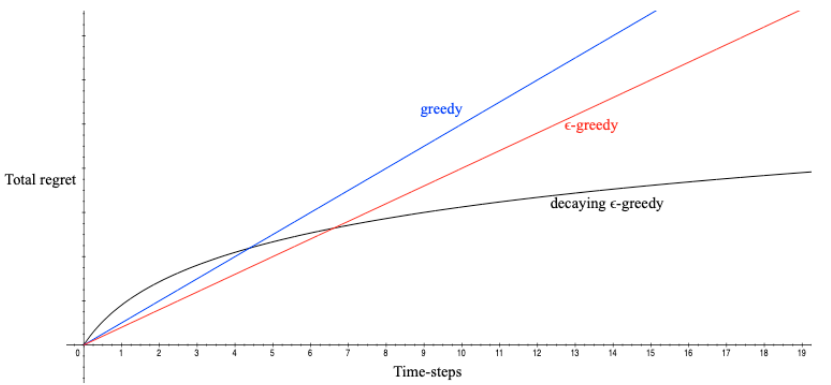
\includegraphics[width=\linewidth]{images/A1.png}
    \label{fig:Scaled Dot Product Attention}
    \vspace{-10pt}
\end{wrapfigure}
Infine, è importante osservare che né un'esplorazione infinita né un completo abbandono dell'esplorazione portano a buone prestazioni. Un algoritmo che continua ad esplorare per sempre accumulerà un regret lineare nel tempo, mentre un algoritmo che non esplora affatto rischia di convergere su un'azione sub-ottimale, anch'esso con regret lineare. Il punto cruciale del problema del multi-armed bandit è proprio determinare se e come sia possibile ottenere un regret sublineare nel tempo, cioè crescere più lentamente di $t$, dimostrando così che l'agente impara effettivamente a comportarsi in modo vicino all'ottimo.

\subsection{Greedy Algorithm}

Per affrontare il problema del multi-armed bandit, una prima classe di algoritmi consiste nello stimare il valore di ciascuna azione mediante valutazione Monte Carlo. L'idea è quella di costruire una stima $\hat{Q}_t(a)$ del valore reale $Q(a)$ a partire dai reward osservati. Per ogni azione $a$, la stima viene aggiornata come media dei reward ottenuti ogni volta che tale azione è stata selezionata. Formalmente, se indichiamo con $N_t(a)$ il numero di volte in cui l'azione $a$ è stata scelta entro il tempo $t$, allora la stima Monte Carlo è:
\[
\hat{Q}_t(a) = \frac{1}{N_t(a)} \sum_{\tau = 1}^{t} r_{\tau} \, \mathbf{1}(a_\tau = a),
\]
dove $\mathbf{1}(\cdot)$ è la funzione indicatrice che vale $1$ quando l'azione al tempo $\tau$ coincide con $a$ e $0$ altrimenti.

Sulla base di questa stima, l'algoritmo \emph{greedy} sceglie semplicemente l'azione che al tempo $t$ presenta il valore stimato più alto. In altre parole, l'azione selezionata è:
\[
a_t^* = \arg\max_{a \in \mathcal{A}} \hat{Q}_t(a).
\]
Questo approccio sfrutta sempre l'informazione disponibile al meglio, scegliendo l'azione che sembra la migliore sulla base dei dati raccolti finora. Tuttavia, il comportamento greedy presenta un limite cruciale: se inizialmente un'azione sub-ottimale riceve per caso reward leggermente migliori, lo stimatore potrebbe sovrastimarne il valore, inducendo l'agente a selezionarla ripetutamente. In questo modo l'algoritmo può ``bloccarsi'' su un'azione non ottimale, senza esplorare sufficientemente le alternative.

L'algortimo greedy ha un total regret \textbf{lineare.}

\subsection{Optimistic Initialization}
Un modo semplice per favorire l'esplorazione è inizializzare le stime dei valori delle azioni a un valore molto alto, tipicamente $\hat{Q}_t(a) = r_{\max}$ per ogni azione $a$. Con tutte le azioni inizialmente valutate come ottimali, l'agente, pur agendo in modo greedy,
\[
a_t = \arg\max_a \hat{Q}_t(a),
\]
finisce per esplorarle tutte almeno una volta.

Tuttavia, questa spinta all'esplorazione è solo iniziale: man mano che le stime vengono aggiornate, i valori $\hat{Q}_t(a)$ scendono verso le loro medie reali e l'algoritmo diventa rapidamente equivalente a un greedy puro, senza più alcun meccanismo di esplorazione. Di conseguenza, poche osservazioni sfortunate possono far scartare definitivamente un'azione ottimale, e anche l'optimistic initialization porta a un regret totale lineare nel tempo.

\subsection{$\varepsilon$-Greedy e $\varepsilon_t$-Decaying}

Un modo semplice per mantenere l'esplorazione continua nel problema del multi-armed bandit è l'algoritmo $\varepsilon$-greedy. In questo approccio, ad ogni passo l'agente:

\begin{compactitemize}
    \item con probabilità $1-\varepsilon$ seleziona l'azione con valore stimato più alto,
    \[
    a = \arg\max_{a \in \mathcal{A}} \hat{Q}_t(a),
    \]
    \item con probabilità $\varepsilon$ sceglie un'azione a caso tra tutte le possibili.
\end{compactitemize}

In questo modo, l'algoritmo continua a esplorare indefinitamente. La scelta di un $\varepsilon$ costante garantisce che il regret istantaneo abbia un limite inferiore:
\[
l_t \ge \frac{\varepsilon}{|\mathcal{A}|} \sum_{a \in \mathcal{A}} \Delta_a,
\]
e quindi il regret totale rimane lineare nel tempo.

Per ridurre il regret nel lungo periodo, è possibile utilizzare una versione con $\varepsilon$ decrescente nel tempo, detta $\varepsilon_t$-greedy. In questo caso si sceglie una sequenza $\varepsilon_1, \varepsilon_2, \dots$ decrescente, ad esempio:
\[
\varepsilon_t = \min \left\{ 1, \frac{c|\mathcal{A}|}{d^2 t} \right\}, \quad c>0, \quad d = \min_{a:\Delta_a>0} \Delta_a,
\]
così che all’inizio l’agente esplori molto e poi gradualmente si comporti in modo quasi greedy. Con questa scelta di decrescita, il regret totale asintotico cresce solo in modo logaritmico con il tempo.

Tuttavia, questo schema richiede di conoscere a priori i gap $\Delta_a$, il che non è realistico nella maggior parte dei casi. L’obiettivo rimane quindi trovare algoritmi capaci di garantire un regret sublineare senza conoscenze preliminari sulle differenze di valore tra le azioni.

\subsection{Lower Bound of Regret}

La difficoltà del problema dipende dalla similarità tra l'azione ottimale e le azioni sub-ottimali. Quando due azioni generano reward con distribuzioni molto simili, l'agente deve raccogliere molte osservazioni per distinguerle, e questo porta inevitabilmente ad accumulare regret. Tale similarità è descritta dalla divergenza di Kullback–Leibler tra le distribuzioni dei reward:
\[
KL(R_a \,\|\, R_{a^*}).
\]

Il teorema classico di Lai e Robbins mostra che ogni algoritmo coerente deve subire un regret almeno logaritmico nel tempo. In particolare:
\[
\lim_{t \to \infty} L_t \;\ge\; \log t \sum_{a:\,\Delta_a>0} \frac{\Delta_a}{KL(R_a \,\|\, R_{a^*})}.
\]

Questo limite indica che il costo dell'esplorazione è inevitabile: per distinguere correttamente le azioni, un algoritmo deve selezionare le azioni sub-ottimali un numero di volte che cresce almeno come $\log t$, rendendo impossibile ottenere regret sub-logaritmico.

\subsection{Optimism in the Face of Uncertainty}

Nel contesto del multi-armed bandit, il principio dell'\emph{Optimism in the Face of Uncertainty} stabilisce che, quando dobbiamo scegliere tra più azioni, dovremmo preferire quelle sulle quali abbiamo maggiore incertezza. L'idea è che un'azione poco esplorata potrebbe in realtà avere un valore molto più alto di quanto stimato finora, e quindi vale la pena indagarla meglio.
\begin{figure}[H]
    \centering
    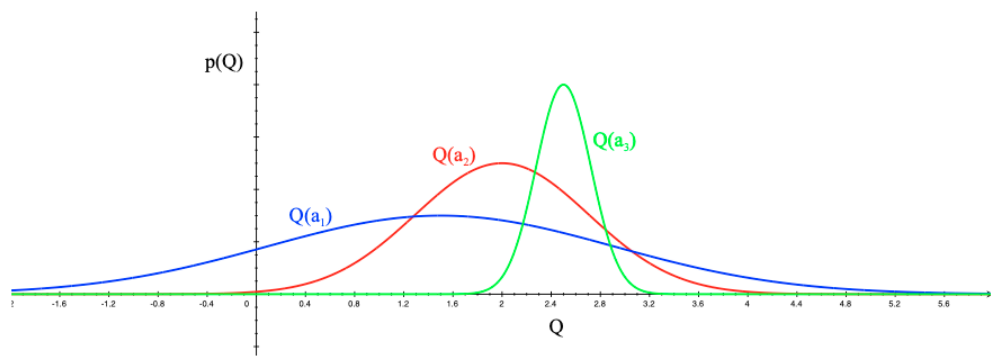
\includegraphics[width=0.6\textwidth]{images/A2.png}
    \label{fig:student_markov_chain}
\end{figure}
Nell'immagine iniziale sono mostrate tre azioni, ciascuna rappresentata da una distribuzione di probabilità sul valore atteso del reward. La curva verde rappresenta un'azione che, secondo le informazioni correnti, sembra avere un valore atteso più alto; la curva rossa un’azione plausibilmente intermedia; mentre quella blu è molto incerta, cioè molto più larga rispetto alle altre. Una distribuzione più larga indica che abbiamo pochi dati su quell'azione, quindi la nostra stima del suo valore è imprecisa.

Il punto centrale dell'approccio ottimistico è proprio questo: un'azione con alta incertezza potrebbe rivelarsi migliore di quanto stimato. Per questo motivo l'algoritmo sceglie di esplorare l'azione blu, nonostante attualmente sembri peggiore di quella verde. Questa scelta “ottimistica” deriva dal considerare non solo il valore atteso stimato, ma anche l’incertezza attorno a tale stima.
\begin{figure}[H]
    \centering
    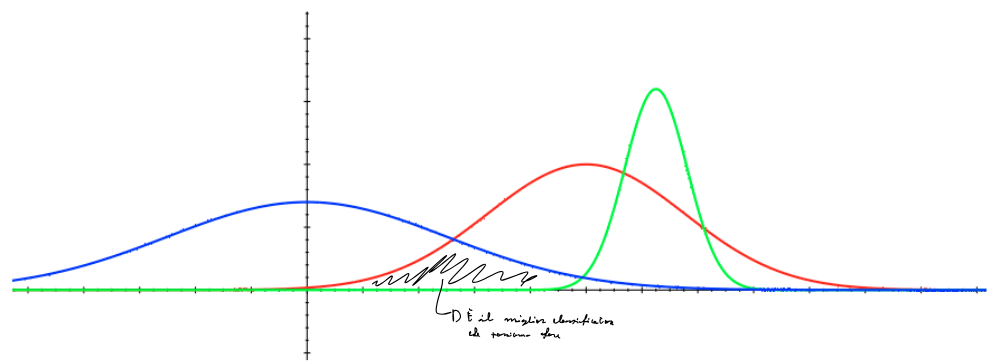
\includegraphics[width=0.6\textwidth]{images/A3.png}
    \label{fig:student_markov_chain}
\end{figure}
Nella seconda immagine vediamo cosa accade dopo aver selezionato l’azione più incerta (la blu). Avendola campionata, la distribuzione si restringe: ora conosciamo meglio il suo valore e quindi siamo meno incerti su di essa. Questa riduzione dell'incertezza elimina la porzione della distribuzione blu che poteva superare le altre, rendendo meno probabile sceglierla nuovamente. Di conseguenza, l’algoritmo inizierà a esplorare altre azioni, come la rossa, continuando questo processo finché non individua l’azione che effettivamente offre il miglior valore atteso.

In sintesi, l’ottimismo di fronte all’incertezza guida l’esplorazione in modo intelligente: selezioniamo le azioni non solo in base alla stima attuale dei loro valori, ma anche in base alla possibilità che queste stime siano troppo conservative. Esplorando sistematicamente le azioni più incerte, l’agente riesce a distinguere meglio tra le diverse distribuzioni di reward e a convergere sull’azione ottimale.

\subsection{Upper Confidence Bounds (UCB)}

L'idea alla base degli \emph{Upper Confidence Bounds} è quella di stimare non solo il valore medio di un'azione, ma anche un intervallo di confidenza entro cui tale valore potrebbe trovarsi. Poiché la nostra stima $Q_t(a)$ è basata su un numero limitato di osservazioni, essa è soggetta a incertezza. Per questo motivo definiamo un termine di confidenza $U_t(a)$ tale che, con alta probabilità,
\[
q(a) \le Q_t(a) + U_t(a).
\]

Questo intervallo dipende fortemente dal numero di volte $N_t(a)$ in cui l'azione $a$ è stata selezionata:
\begin{compactitemize}
    \item se $N_t(a)$ è piccolo, allora $U_t(a)$ è grande: significa che conosciamo poco l'azione e la stima è molto incerta;
    \item se $N_t(a)$ è grande, allora $U_t(a)$ è piccolo: la nostra stima di $Q_t(a)$ è più affidabile.
\end{compactitemize}

Seguendo il principio dell'ottimismo nell'incertezza, l'agente seleziona l'azione che massimizza la somma tra valore stimato e banda di confidenza:
\[
a_t = \arg\max_a \left( Q_t(a) + U_t(a) \right).
\]

Questo permette di bilanciare automaticamente esplorazione e sfruttamento: le azioni meno esplorate avranno $U_t(a)$ maggiore e quindi verranno selezionate più spesso.

\subsection{Hoeffding's Inequality}

Per costruire concretamente il termine di confidenza $U_t(a)$ utilizziamo la disuguaglianza di Hoeffding. Siano $X_1, \dots, X_t$ variabili i.i.d.\ in $[0,1]$ e sia
\[
\bar{X}_t = \frac{1}{t} \sum_{\tau=1}^t X_\tau
\]
la media campionaria. Hoeffding garantisce che
\[
\mathbb{P}\!\left( \mathbb{E}[X] > \bar{X}_t + u \right) \le e^{-2tu^2},
\]
cioè la probabilità che il valore atteso superi la stima empirica più $u$ decresce esponenzialmente con il numero di osservazioni.

Applicando questa disuguaglianza al reward di un'azione $a$ condizionato sulla selezione di tale azione otteniamo:
\[
\mathbb{P}\!\left( q(a) > Q_t(a) + U_t(a) \right)
\le e^{-2 N_t(a)\, U_t(a)^2}.
\]

Questa è l’intuizione matematica che ci permette di costruire una banda di confidenza in modo rigoroso.

\subsection{Calcolo della Banda di Confidenza}

Per calcolare $U_t(a)$ scegliamo una probabilità $p$ che rappresenti il rischio che il valore reale superi la banda di confidenza. Impostiamo:
\[
e^{-2 N_t(a)\, U_t(a)^2} = p.
\]

Risolviamo rispetto a $U_t(a)$:
\[
U_t(a) = \sqrt{\frac{-\log p}{2N_t(a)}}.
\]

Possiamo far variare $p$ nel tempo, ad esempio ponendolo come funzione $p=f(t)$ che diminuisce all'aumentare del numero di osservazioni. In questo modo, man mano che raccogliamo dati, l'intervallo di confidenza si restringe e l'algoritmo converge verso l'azione ottimale.

\subsection{UCB1}

Utilizzando come scelta $p = t^{-4}$ otteniamo una forma particolarmente semplice ed efficace, che dà origine all'algoritmo \textbf{UCB1}. In questo caso la banda di confidenza diventa:
\[
U_t(a) = \sqrt{\frac{2\log t}{N_t(a)}},
\]
e la regola di selezione delle azioni risulta:
\[
a_t = \arg\max_a \left[ Q_t(a) + \sqrt{\frac{2\log t}{N_t(a)}} \right].
\]

L'algoritmo UCB1 garantisce un regret totale asintotico logaritmico:
\[
\lim_{t \to \infty} L_t \le 
8 \log t \sum_{a : \Delta_a > 0} \frac{1}{\Delta_a}.
\]

Questo risultato è notevole perché raggiunge (a costanti moltiplicative) il lower bound di Lai e Robbins, rendendo UCB uno degli algoritmi ottimali per il problema del multi-armed bandit.

\subsection{Bayesian Bandits}

Finora non abbiamo fatto alcuna assunzione sulla forma delle distribuzioni di reward. I \emph{Bayesian bandits}, invece, sfruttano conoscenza a priori sulle distribuzioni dei reward.  
L’idea è quella di modellare il valore delle azioni tramite un insieme di parametri $\mathbf{w}$, ad esempio assumendo che ogni azione abbia una distribuzione gaussiana indipendente con media e varianza ignote:
\[
\mathbf{w} = [\mu_1, \sigma_1^2, \dots, \mu_k, \sigma_k^2].
\]

A partire da un prior $p(\mathbf{w})$ e dai reward osservati, possiamo calcolare la distribuzione a posteriori al tempo $t$:
\[
p(Q(a)\mid h_t) = p(Q(a)\mid \mathbf{w})\, p(\mathbf{w} \mid h_t),
\]
dove $h_t$ rappresenta la storia delle osservazioni fino al tempo $t$.

La conoscenza a posteriori viene poi utilizzata per guidare l’esplorazione. Due metodi molto comuni sono:

\begin{compactitemize}
    \item \textbf{Bayesian UCB}: utilizza la distribuzione a posteriori per costruire una stima ottimistica del valore;
    \item \textbf{Probability Matching}: seleziona un’azione in proporzione alla probabilità che sia ottimale.
\end{compactitemize}

Se il prior è accurato, i Bayesian bandits possono ottenere prestazioni migliori rispetto ai metodi frequentisti.

\begin{figure}[H]
    \centering
    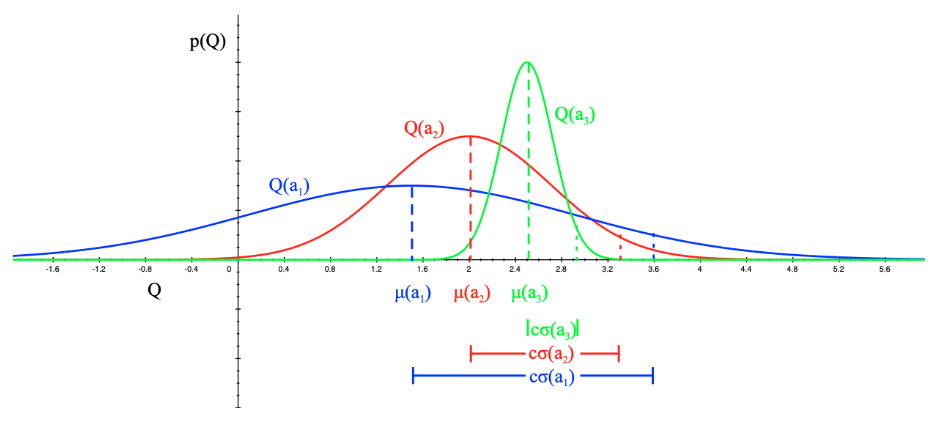
\includegraphics[width=0.8\textwidth]{images/A4.png}
    \label{fig:student_markov_chain}
\end{figure}
\subsection{Bayesian UCB}

Consideriamo il caso in cui le distribuzioni dei reward siano gaussiane:
\[
R_a(r) = \mathcal{N}(r; \mu_a, \sigma_a^2).
\]

Utilizzando la legge di Bayes, possiamo calcolare la distribuzione a posteriori sui parametri $\mu_a$ e $\sigma_a^2$ combinando il prior con i reward osservati. La distribuzione a posteriori del valore di un’azione $a$ ha quindi una deviazione standard $\sigma_a$ che misura l’incertezza residua.

L’idea del \emph{Bayesian UCB} è quella di costruire un limite superiore di confidenza direttamente dalla posterior:
\[
U_t(a) = c\, \sigma_a,
\]
dove $c$ è un parametro che controlla quanto essere “ottimisti”.

L’azione selezionata è quindi:
\[
a_t = \arg\max_a \left( Q_t(a) + c\, \sigma_a \right).
\]

In questo modo, un’azione molto incerta (varianza alta) riceve un aumento maggiore del proprio valore stimato e viene scelta più spesso, coerentemente con il principio dell’ottimismo nell’incertezza.

\subsection{Probability Matching}

Il \emph{Probability Matching} seleziona l’azione $a$ in proporzione alla probabilità che essa sia realmente l’azione ottimale. Formalmente:
\[
\pi(a) = \mathbb{P}\!\left( Q(a) = \max_{a'} Q(a') \,\middle|\, R_1, \dots, R_{t-1} \right).
\]

Questo metodo è naturalmente ottimista: se un’azione è molto incerta, la posterior assegna una probabilità non trascurabile che possa essere la migliore, e quindi quell’azione verrà selezionata più spesso. Tuttavia, calcolare esattamente queste probabilità può essere difficile in modo analitico.

\subsection{Thompson Sampling}

Il \emph{Thompson Sampling} è una versione campionata del probability matching. L’idea è molto semplice:

\begin{enumerate}
    \item Si calcola la distribuzione a posteriori $p(\mathbf{w}\mid R_1,\dots,R_{t-1})$ tramite la legge di Bayes.
    \item Si estrae un campione di una funzione valore $Q(a)$ dalla posterior.
    \item Si seleziona l’azione con il valore più alto nel campione:
    \[
    a_t = \arg\max_a Q(a).
    \]
\end{enumerate}

Ripetendo questo schema a ogni passo, la probabilità di selezionare un’azione coincide con la probabilità che essa sia ottimale secondo il posterior: questo realizza esattamente il probability matching in modo semplice ed efficiente.

Un risultato fondamentale è che il Thompson Sampling raggiunge il lower bound di Lai e Robbins nei bandit di tipo Bernoulli, risultando quindi ottimalmente efficiente dal punto di vista del regret asintotico.

